% Include the temperature and pressure history of the cure cycle in the report.
After the layup phase is completed, the curing process can begin. In general, the curing process involves exposing the specimen to high temperatures and pressures. Both the magnitude and duration of the elevated temperatures and pressures influence the quality of the final specimen. Different materials require different cure cycle characteristics for optimal results. A typical cure cycle can be divided in two major steps: the consolidation stage and the cure stage. During the consolidation stage, heat is applied to reach an intermediate temperature and pressure is applied. The heat reduces the viscosity of the resin and the pressure squeezes excess resin out of the laminate. The pressure also "consolidates" the individual specimen plies and removes voids.  During the cure stage, the temperature is elevated even more. The higher temperature initiates resin polymerization and produces cross-linking. 

\begin{figure}[H]
    \centering
    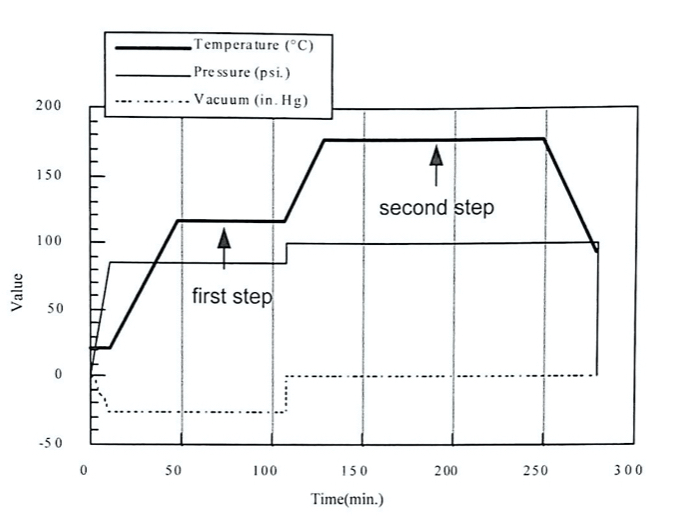
\includegraphics[width=0.8\textwidth]{Pictures/Lab1: Q 1.10/typical_cure.jpg}
    \caption{Typical Cure Cycle\cite{labmanual}}
    \label{fig:typicalcure}
\end{figure}

Figure \ref{fig:typicalcure} displays the temperatures and pressures in a typical cure cycle. Here, the difference in temperatures and pressures between the first and second steps can be seen. Note that this figure corresponds to a typical cure cycle, and not the one used for this lab.

For this lab, a single step cure cycle is used. In this case, the temperature and pressure are raised to a predetermined value only once. Figure \ref{fig:mariecuring} displays the curing cycle for the specimen used in this lab. The single step, as opposed to two steps in the cycle discussed earlier, can be seen in this figure.

